\section{Durchführung}
\label{sec:Durchführung}
Für die Durchführung dieses Versuches werden zwei Proben instabiler Isotope benötigt. Dieses Versuchsprotokoll befasst sich mit den Isotopen $\ce{^{52}_{23}V}$ und 
$\ce{^{104}_{45}}$. Beide Isotope müssen, bevor der Verusch durchgeführt werden kann, durch Neutronenbestrahlung \textit{aktiviert} werden. Dies geschieht in einem dafür
konstruierten Behälter. $\ce{^{104}_{45}}$ muss sich für mindestens $\qty{20}{\minute}$ in diesem Behälter befinden, bevor damit eine Messung durchgeführt werden kann. 
$\ce{^{52}_{23}V}$ muss lediglich $\qty{15}{\minute}$ reaktiviert werden. Sind die Proben einsatzbereit werden diese in die Messapparatur eingesetzt, welche in
\autoref{fig:Messapparatur} dargestellt wird.  

\begin{figure}
    \centering
    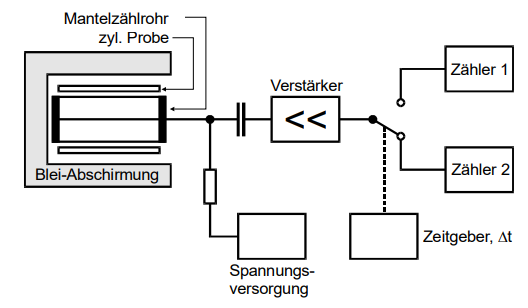
\includegraphics[width = .7\textwidth]{content/Skizzeapparatur.png}
    \caption{In dieser Abbildung ist der Aufbau der verwendeten Messapparatur skizziert. \cite{v702}}
    \label{fig:Messapparatur}
\end{figure}

Bevor die Messungen begonnen werden können wird die \textit{Nullzählrate} des Zählrohrs bestimmt. Dazu darf keine Probe in das Zählrohr eingeführt werden. Dann wird eine Messung 
über $\qty{600}{second}$ durchgeführt. Dabei wird nur über einen Zähler eine Messung aufgenommen. Der daraus resultierende Messwert wird als Hintergundrauschen für die weiteren
Messungen verwendet.

Die Messung wird nun mit dem Rhodium-Isotrop begonnen. Dazu wird die Probe in das Zählrohr eingeführt und an dem \textit{Zählgerät} wird ein Messzeitintervall 
$\symup{\Delta}t = \qty{15}{\second}$ eingestellt. Das Zählgerät besitzt zwei Zähler. Nach dem Durchlauf eines Messzeitintervalls schlägt der eingebaute Schalter um und der 
andere Zähler läuft weiter. Durch dieses Verfahren werden für Rhodium mit einem Messzeitintervall von $\symup{\Delta}t = \qty{15}{\second}$ $\num{15}$-mal durchgeführt. Das 
ergibt eine Gesamtzählzeit von $\qty{12}{\minute}$. Dabei werden die Zählraten der Messzeitintervalle notiert. 

Nun wird ein Vanadium-Isotop $\left(\ce{^{52}_{23}V}\right)$ verwendet. Die Messung wird vom Konzept exakt identisch durchgeführt. Allerdings muss bei dem Vanadium-Isotop
darauf geachtet werden, dass es mindestens $\qty{15}{\minute}$ aktiviert wird bevor es zu einer Messung verwendet wird. Außerdem werden nun Messzeitintervalle von 
$\symup{\Delta}t = \qty{30}{\second}$ verwendet und die Messreihe wird über eine Gesamtzählzeit von $\qty{15}{\minute}$ aufgenommen.
